\documentclass{beamer}
%\usepackage{bookman} % importa a bookman family font para
%ser usado na apresentação

\title{Titulo}
\subtitle{Algum subtítulo}
\author[Marco, DKM]{Marco Henry\inst{1} \and Danilo Kotaka\inst{2}}
\institute[UEL]{Universidade Estadual De Londrina}
\date{\today}

\AtBeginSection[]
{
	\begin{frame}
		\frametitle{Sumário}
		\tableofcontents
	\end{frame}
}

\usetheme{Szeged}
%\usecolortheme{}
%\usefonttheme{structuresmallcapsserif}

\begin{document}
	
	\frame{\titlepage}
	
	\begin{frame}
		\frametitle{Orquestração e Auto-scaling em Nuvem}
		\begin{columns}
			\column{1\textwidth}
			A Computação Autônoma atua como o motor de orquestração essencial para manter a viabilidade econômica dos provedores modernos.
			\begin{itemize}
			\item{\textbf{Auto-otimização:}}Provisionamento dinâmico (auto-scaling) baseado em métricas de CPU e latência em tempo real. Economizando energia e custo.
			\item{\textbf{Eficiência Energética:}} Consolidação de cargas de trabalho e desligamento de recursos ociosos.
			\item{\textbf{Resiliência:}}Detecção de degradação e migração automática de VMs sem interrupção de serviço. Por meio de migração automática de VMs e reconfiguração de balanceadores.
			\end{itemize}
		\end{columns}
	\end{frame}
	\begin{frame}
		\frametitle{Orquestração e Auto-scaling em Nuvem}
		\begin{figure}
			\centering
			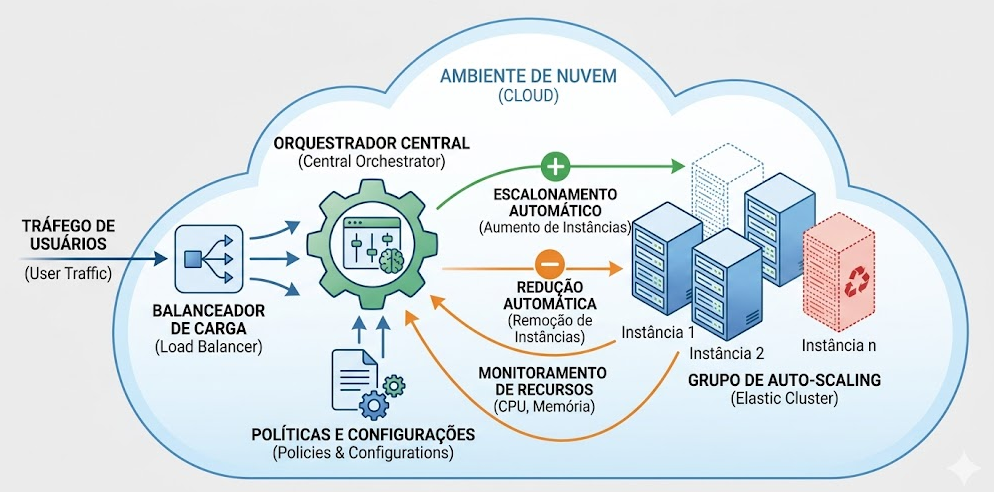
\includegraphics[scale=0.3]{./images/orquestracao_nuvem.png}	
			\caption{Funcionamento da orquestração em nuvem}
		\end{figure}
	\end{frame}
	
	\begin{frame}
		\frametitle{Sistemas Pervasivos e IoT}
		\begin{itemize}
			\item Desafio: heterogeneidade + volatilidade + recursos limitados.
			\item Auto-configuração: dispositivos plug-and-play em Smart Cities e Smart Grids. Descobrem vizinhos e registram serviços automaticamente.
			\item Auto-proteção: detecção de tráfego anômalo (DDoS, intrusões) e quarentena automática de dispositivos comprometidos.
			\item Sem autonomia, o custo de configurar milhões de sensores seria proibitivo.
		\end{itemize}
	\end{frame}

	\begin{frame}
		\frametitle{Estado da Arte: Mudança de Paradigma}
		A pesquisa não busca mais justificar a autonomia, mas refinar o MAPE-K e resolver suas limitações.
		
		Principal mudança no método foi sair de regras estáticas para para a autonomia preditiva com IA/ML.
		\begin{itemize}
			\item Aprendizado por Reforço e Redes Neurais Profundas substituem políticas estáticas se-então.
			\item O sistema aprende políticas ótimas por tentativa e erro ou via dados históricos.
		\end{itemize}
	\end{frame}
	
	\begin{frame}
		\frametitle{Paradigmas Industriais Consolidados}
		AiOps (AIOps (Artificial Intelligence for IT Operations))
		\begin{itemize}
			\item Estado da arte em auto-cura e auto-otimização de data centers.
			\item Ingere terabytes de logs/métricas e antecipa falhas horas antes de ocorrerem.
		\end{itemize}
		Orquestração Cloud-Native \& Service Mesh
		\begin{itemize}
			\item Microsserviços adotam Self-X de forma nativa.
			\item Kubernetes + Service Mesh → auto-configuração e auto-cura em milissegundos.
		\end{itemize}
	\end{frame}
	
	\begin{frame}
		\frametitle{Lacunas e Desafios em Aberto}
		\begin{enumerate}
			\item Verificação Formal e Estabilidade
			Problema da ``caixa-preta'' do ML → necessidade de provar matematicamente a corretude.
			
			\item Interoperabilidade \& Sistemas Multi-agente
			Soluções atuais vivem em silos; falta padronização para troca de conhecimento entre gerentes autônomos.
			
			\item Tradução de Políticas de Alto Nível
			Converter metas de negócio ("maximizar lucro minimizando latência") em ações operacionais ainda exige especialista humano.
		\end{enumerate}
		
		Fronteira atual: tornar a autonomia verificável, interpretável e interoperável.
	\end{frame}
	
	\begin{frame}
		\frametitle{Conclusão}
		\begin{itemize}
			\item A escalabilidade da TI moderna não pode mais ser dissociada da automação de sua gestão.
			\item A capacidade cognitiva humana é o principal limitador das infraestruturas contemporâneas.
			\item A "crise da complexidade" é o desafio central. A Computação Autônoma é a resposta.
			\item As propriedades Self-CH, sustentadas pelo MAPE-K, viabilizam Cloud, IoT e sistemas pervasivos não apenas tecnicamente, mas economicamente (redução de TCO + cumprimento de SLAs).
		\end{itemize}
	\end{frame}
	
	\begin{frame}
		\frametitle{Conclusão}
		
		A transição de sistemas que auxiliam decisões → para sistemas que agem sozinhos ainda esbarra em:
		\begin{itemize}
			\item Interoperabilidade entre fornecedores
			\item Confiança dos administradores
			\item Estabilidade formal dos algoritmos
		\end{itemize}
		
		Em uma era de trilhões de dispositivos, autonomia deixa de ser diferencial e passa a ser requisito mandatório.
	\end{frame}
\end{document}
